\documentclass[11pt]{report}

\textheight=23cm \textwidth=16cm
\topmargin=-1cm
\oddsidemargin=0pt \evensidemargin=0pt \marginparwidth=2cm

\usepackage{psfig}

\newcommand{\T}[1]{{\tt #1}}

\title{Metanet Tutorial}
\author{Claude Gomez \and Maurice Goursat}
\date{14 July 1995}

\makeindex

\begin{document}

\maketitle

Metanet is a toolbox of Scilab. In fact, it is a toolbox of Scilab
with another software linked to Scilab: XMetanet.

The Scilab toolbox consists of fortran and C programs and Scilab
macros.  
They give a set of Scilab functions dealing with graph and
network computations. A new object, a graph-list is defined in Scilab to handle
graph.

XMetanet is a X Window application for creating, modifying and
vizualizing graphs and networks. XMetanet and Scilab can be
used separately. 

 The first chapter is a tutorial which explains
how to use the Metanet toolbox of Scilab.
 The second chapter describes explains how to use the X
Window application XMetanet.
 The third chapter describes the structure of the
graph-list.
 The last chapter describes all the functions
of the toolbox.

\chapter{Using Metanet}

You can use the Metanet toolbox in Scilab without using XMetanet window at
all,
\mbox{i.e.} without seeing the graphs or the networks you are working with,
even if it seems better to use XMetanet to see them. You only need to use 
XMetanet when you want to see graphs, or when you want to load already 
saved graph.
So, a good thing to do before using Metanet
is to open a Metanet window, \mbox{i.e.} to execute the X Window application
XMetanet from Scilab. For that, use the Metanet Menu in
Scilab. It is exactly the same as issuing the command \T{metanet()}.

\section{Creating and Loading Graphs}

A graph in Scilab is defined by a list: we call it a
{\em graph-list}. It  
is described in \ref{graph-list}. This list contains everything needed to
define the graph, from the arcs and nodes to the color and width of the
arcs. We are going to see it is not necessary to fill of the elements of
the list; for most of them defaults are given.

To create a new graph in Scilab, you can make a new graph-list or make the
graph by using XMetanet and load it. We describe her
the first way: make a new graph-list. For the second way, see \ref{XMetanet}.
For making a graph-list, use the
\T{make\_graph} function.

For instance, the directed graph named ``foo'' in figure~\ref{fig-small}
has three nodes and four
arcs. We call \T{g} the corresponding graph-list.

\begin{figure}
  \centerline{\psfig{file=graph1.ps,angle=-90}}
  \caption{Small directed graph}
  \label{fig-small}
\end{figure}

You can easily create it by issuing the command:

\begin{verbatim}
g=make_graph('foo',1,3,[1,2,3,1],[2,3,1,3]);
\end{verbatim}

The first argument is the name of the graph,
the second argument \T{1} says that the graph is directed, the third
and fourth arguments are what we call tail
and head
vectors of 
the graph and the last argument is the number of nodes of the graph.

To understand this, we need to explain how a graph is represented.

The graphs handled by Metanet are directed or undirected multigraphs 
(loops are allowed). 
A {\em graph}\index{graph}
is a set of arcs and nodes. A graph must at least have one arc. 
We call {\em arc}\index{arc} a directed link between two nodes. 
For instance the arc $(i,j)$ goes from the {\em tail}\index{tail}
node $i$ to the {\em head}\index{head}
node $j$. 
We call {\em edge}\index{edge} the 
corresponding undirected link. A minimal way to represent a graph is to
give the number of nodes, the list of the tail nodes and the list of the
head nodes. Each node has a number and each arc has a number. The numbers
of nodes are consecutive and the number of arcs are consecutive. In Scilab,
these lists are represented by vectors. So, if we call \T{tail} and
\T{head} these vectors, the arc number $i$ goes from node
number \T{tail(i)} to node number \T{head(i)}. Moreover, the number of
nodes is necessary, because isolated nodes (without any arc) can exist. The
size of the vectors tail and head is the number of edges of the graph.

The distinction between edges and arcs is meaningful when we deal with
undirected graphs. In computations, an undirected graph is considered as a
directed graph where each edge of the undirected graph is splitted into two
arcs with consecutive numbers: the edge  number $u$ between nodes $i$ and $j$
becomes the arc  number $2i-1$ from node $i$ to node $j$ and the arc 
 number
$2i$ from node $j$ to node $i$. This distinction is not needed when we
only use the standard functions of Metanet.

The simplest graph we can create in Metanet is:
\begin{verbatim}
g=make_graph('min',1,1,1,1);
\end{verbatim}

It is directed, has one node and one loop arc on this node and can be
seen in figure~\ref{fig-smallest}.
\begin{figure}
  \centerline{\psfig{file=graph2.ps,angle=-90}}
  \caption{Smallest directed graph}
  \label{fig-smallest}
\end{figure}

The following graph shown in figure~\ref{fig-usmall} is the same as
the first graph we have created, but it 
is undirected:
\begin{verbatim}
g=make_graph('foo',0,3,[1,2,3,1],[2,3,1,3]);
\end{verbatim}

\begin{figure}
  \centerline{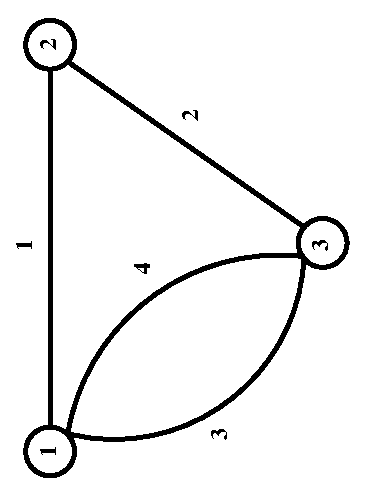
\psfig{file=graph3.ps,angle=-90}}
  \caption{Small undirected graph}
  \label{fig-usmall}
\end{figure}

Next graph shown in figure~\ref{fig-isolated} is directed and has one
isolated node (number 3): 
\begin{verbatim}
g=make_graph('foo',1,4,[1,2,4,1],[2,4,1,4]);
\end{verbatim}

\begin{figure}
  \centerline{\psfig{file=graph4.ps,angle=-90}}
  \caption{Isolated node in directed graph}
  \label{fig-isolated}
\end{figure}

But what about the other elements of the graph-list (see \ref{graph-list})? 
In fact, you do not need to give them if they
are meaningless for your problem or you do not know what to put. Defaults
are given for you. The only needed elements are the arguments of the
\T{make-graph} function:
\begin{description}
  \item[name] the name of the graph
  \item[directed] 0 or 1 according to the fact that the graph is
    respectively undirected or directed
  \item[node\_number] the number of nodes of the graph
  \item[tail] the vector of the  tail node numbers of the graph (its
    size is the number of edges of the graph)
  \item[head] the vector of the head node numbers of the graph (its 
    size is the number of edges of the graph)
\end{description}

and the type \T{'graph'} as the
first element of the list.

All the other elements can be given as the empty vector \T{[]}. Then
defauls are automatically chosen. These defaults are given in the
description of the graph-list (see \ref{graph-list}).

But you can also create your own graph-list by hands, without using the 
\T{make\_graph} function. For that you can use the Scilab function
\T{list}
directly and modify it with the insertion list functions. This way can lead
to errors, because the list is somehow long. You can use the 
\T{check\_graph}
function to check if a Scilab variable can represent a graph-list.

\section{Graph Computations}

\chapter{XMetanet}\label{XMetanet}

\section{Graph Files}

\chapter{Graph List}\label{graph-list}
\index{graph list}
A graph in Scilab is represented by a Scilab typed list with 32 elements. 
We call it a
graph-list.

You will find below the complete description of the list.

Each element is described by two or more lines.
The first line gives the order of the element in the list and its name.
The other lines give the meaning of the element with its Scilab type if
needed.
The last line gives a default for elements that can have one.
Indeed, only the 6 first elements must have a value in the list, all the 
others can be given the empty vector \T{[]} as a value, and then the default 
is used.
For instance, after you have defined a graph-list by
\begin{verbatim}
g=make_graph('min',1,1,1,1);
\end{verbatim}

which is the simplest graph you can create in Metanet (it is directed, has 
one node and one loop arc on this node), the value of \T{g} is:
\begin{verbatim}
list('graph','min',1,1,1,1,[],[],[],[],[],[],[],[],[],[],[],[],[],[],[],
     [],[],[],[],[],[],[],[],[],[],[],[])
\end{verbatim}

The name of the element is very important because it is used to access 
the elements
of the list. For instance, if \T{g} is a graph-list, to get the name
of the graph, you only have to execute:
\begin{verbatim}
g('name')
\end{verbatim}

and if you want to change the name of the graph to \T{'toto'} for
instance, you have to execute: 
\begin{verbatim}
g('name')='toto';
\end{verbatim}

\begin{enumerate}
  \item \T{type}

the type of the list; it must always be \T{'graph'}

  \item \T{name} 

the name of the graph; a string with a maximum of 80 characters

  \item directed 

flag equal to 1 if the graph is directed or equal to 0 is the graph is
undirected 

  \item \T{node\_number}

number of nodes

  \item \T{tail}

vector of the tail node numbers

  \item \T{head}

vector of the head node numbers

  \item \T{node\_name}

vector of node names

default is the node numbers as node names

  \item \T{node\_type}

vector of the node types; the type is an integer from 0 to 2:
\begin{itemize}
  \item[0:] plain node
  \item[1:] sink node
  \item[2:] source node
\end{itemize}


default is 0 (plain node)

  \item \T{node\_x}

vector of the x coordinate of the nodes

default is computed

  \item \T{node\_y}

vector of the y coordinate of the nodes

default is computed

  \item \T{node\_color}

vector of the node colors; 
the color is an integer from 0 to 16:
\begin{itemize}
  \item[0:] black
  \item[1:] navyblue
  \item[2:] blue
  \item[3:] skyblue
  \item[4:] aquamarine
  \item[5:] forestgreen
  \item[6:] green
  \item[7:] lightcyan
  \item[8:] cyan
  \item[9:] orange
  \item[10:] red
  \item[11:] magenta
  \item[12:] violet
  \item[13:] yellow
  \item[14:] gold
  \item[15:] beige
  \item[16:] white
\end{itemize}


default is 0 (black)

  \item \T{node\_diam}

vector of the size of the node diameters in pixels (a node is
drawn as a circle) 

default is the value of element \T{default\_node\_diam}

  \item \T{node\_border}

vector of the size of the node borders in pixels (a node is drawn
as a circle) 

default is the value of element \T{default\_node\_border}

  \item \T{node\_font\_size}

vector of the size of the font used to draw the name of the node; 
you can choose
8, 10, 12, 14, 18 or 24

default is the value of element \T{default\_font\_size}

  \item \T{node\_demand}

vector of the node demands

default is 0

  \item \T{edge\_name}

vector of the edge names

default is the edge numbers as edge names

  \item \T{edge\_color}

vector of the edge colors; 
the color is an integer from 0 to 16 (see \T{node\_color})

default is 0 (black)

  \item \T{edge\_width}

vector of the size of the edge widths in pixels

default is the value of element \T{default\_edge\_width}

  \item \T{edge\_hi\_width}

vector of the size of the highlighted edge widths in pixels

default is the value of element \T{default\_edge\_hi\_width}

  \item \T{edge\_font\_size}

vector of the size of the font used to draw the name of the edge; you
can choose 8, 10, 12, 14, 18 or 24

default is the value of element \T{default\_font\_size}

  \item \T{edge\_length}

vector of the edge lengths

default is 0

  \item \T{edge\_cost}

vector of the edge costs

default is 0

  \item \T{edge\_min\_cap}

vector of the edge minimum capacities

default is 0

  \item \T{edge\_max\_cap}

vector of the edge maximum capacities

default is 0

  \item \T{edge\_q\_weight}

vector of the edge quadratic weights

default is 0

  \item \T{edge\_q\_orig}

vector of the edge quadratic origins

default is 0

  \item \T{edge\_weight}

vector of the edge weights

default is 0

  \item \T{default\_node\_diam}

default size of the node diameters of the graph

default is 20 pixels

  \item \T{default\_node\_border}

default size of the node borders of the graph

default is 2 pixels

  \item \T{default\_edge\_width}

default size of the edge widths of the graph

default is 1 pixel

  \item \T{default\_edge\_hi\_width}

default size of the highlighted edge widths of the graph

default is 3 pixels

  \item \T{default\_font\_size}

default size of the font used to draw the names of nodes and edges

default is 12

\end{enumerate}

\tableofcontents

\listoffigures

\documentclass[11pt]{report}

\textheight=23cm \textwidth=16cm
\topmargin=-1cm
\oddsidemargin=0pt \evensidemargin=0pt \marginparwidth=2cm

\usepackage{psfig}

\newcommand{\T}[1]{{\tt #1}}

\title{Metanet Tutorial}
\author{Claude Gomez \and Maurice Goursat}
\date{14 July 1995}

\makeindex

\begin{document}

\maketitle

Metanet is a toolbox of Scilab. In fact, it is a toolbox of Scilab
with another software linked to Scilab: XMetanet.

The Scilab toolbox consists of fortran and C programs and Scilab
macros.  
They give a set of Scilab functions dealing with graph and
network computations. A new object, a graph-list is defined in Scilab to handle
graph.

XMetanet is a X Window application for creating, modifying and
vizualizing graphs and networks. XMetanet and Scilab can be
used separately. 

 The first chapter is a tutorial which explains
how to use the Metanet toolbox of Scilab.
 The second chapter describes explains how to use the X
Window application XMetanet.
 The third chapter describes the structure of the
graph-list.
 The last chapter describes all the functions
of the toolbox.

\chapter{Using Metanet}

You can use the Metanet toolbox in Scilab without using XMetanet window at
all,
\mbox{i.e.} without seeing the graphs or the networks you are working with,
even if it seems better to use XMetanet to see them. You only need to use 
XMetanet when you want to see graphs, or when you want to load already 
saved graph.
So, a good thing to do before using Metanet
is to open a Metanet window, \mbox{i.e.} to execute the X Window application
XMetanet from Scilab. For that, use the Metanet Menu in
Scilab. It is exactly the same as issuing the command \T{metanet()}.

\section{Creating and Loading Graphs}

A graph in Scilab is defined by a list: we call it a
{\em graph-list}. It  
is described in \ref{graph-list}. This list contains everything needed to
define the graph, from the arcs and nodes to the color and width of the
arcs. We are going to see it is not necessary to fill of the elements of
the list; for most of them defaults are given.

To create a new graph in Scilab, you can make a new graph-list or make the
graph by using XMetanet and load it. We describe her
the first way: make a new graph-list. For the second way, see \ref{XMetanet}.
For making a graph-list, use the
\T{make\_graph} function.

For instance, the directed graph named ``foo'' in figure~\ref{fig-small}
has three nodes and four
arcs. We call \T{g} the corresponding graph-list.

\begin{figure}
  \centerline{\psfig{file=graph1.ps,angle=-90}}
  \caption{Small directed graph}
  \label{fig-small}
\end{figure}

You can easily create it by issuing the command:

\begin{verbatim}
g=make_graph('foo',1,3,[1,2,3,1],[2,3,1,3]);
\end{verbatim}

The first argument is the name of the graph,
the second argument \T{1} says that the graph is directed, the third
and fourth arguments are what we call tail
and head
vectors of 
the graph and the last argument is the number of nodes of the graph.

To understand this, we need to explain how a graph is represented.

The graphs handled by Metanet are directed or undirected multigraphs 
(loops are allowed). 
A {\em graph}\index{graph}
is a set of arcs and nodes. A graph must at least have one arc. 
We call {\em arc}\index{arc} a directed link between two nodes. 
For instance the arc $(i,j)$ goes from the {\em tail}\index{tail}
node $i$ to the {\em head}\index{head}
node $j$. 
We call {\em edge}\index{edge} the 
corresponding undirected link. A minimal way to represent a graph is to
give the number of nodes, the list of the tail nodes and the list of the
head nodes. Each node has a number and each arc has a number. The numbers
of nodes are consecutive and the number of arcs are consecutive. In Scilab,
these lists are represented by vectors. So, if we call \T{tail} and
\T{head} these vectors, the arc number $i$ goes from node
number \T{tail(i)} to node number \T{head(i)}. Moreover, the number of
nodes is necessary, because isolated nodes (without any arc) can exist. The
size of the vectors tail and head is the number of edges of the graph.

The distinction between edges and arcs is meaningful when we deal with
undirected graphs. In computations, an undirected graph is considered as a
directed graph where each edge of the undirected graph is splitted into two
arcs with consecutive numbers: the edge  number $u$ between nodes $i$ and $j$
becomes the arc  number $2i-1$ from node $i$ to node $j$ and the arc 
 number
$2i$ from node $j$ to node $i$. This distinction is not needed when we
only use the standard functions of Metanet.

The simplest graph we can create in Metanet is:
\begin{verbatim}
g=make_graph('min',1,1,1,1);
\end{verbatim}

It is directed, has one node and one loop arc on this node and can be
seen in figure~\ref{fig-smallest}.
\begin{figure}
  \centerline{\psfig{file=graph2.ps,angle=-90}}
  \caption{Smallest directed graph}
  \label{fig-smallest}
\end{figure}

The following graph shown in figure~\ref{fig-usmall} is the same as
the first graph we have created, but it 
is undirected:
\begin{verbatim}
g=make_graph('foo',0,3,[1,2,3,1],[2,3,1,3]);
\end{verbatim}

\begin{figure}
  \centerline{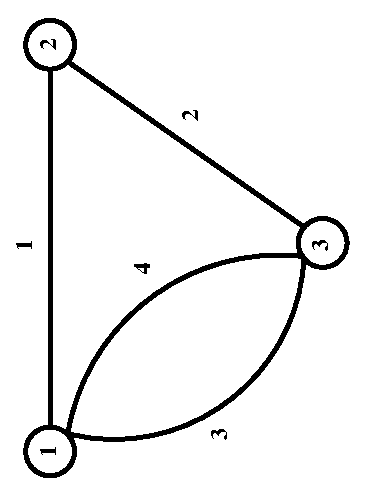
\psfig{file=graph3.ps,angle=-90}}
  \caption{Small undirected graph}
  \label{fig-usmall}
\end{figure}

Next graph shown in figure~\ref{fig-isolated} is directed and has one
isolated node (number 3): 
\begin{verbatim}
g=make_graph('foo',1,4,[1,2,4,1],[2,4,1,4]);
\end{verbatim}

\begin{figure}
  \centerline{\psfig{file=graph4.ps,angle=-90}}
  \caption{Isolated node in directed graph}
  \label{fig-isolated}
\end{figure}

But what about the other elements of the graph-list (see \ref{graph-list})? 
In fact, you do not need to give them if they
are meaningless for your problem or you do not know what to put. Defaults
are given for you. The only needed elements are the arguments of the
\T{make-graph} function:
\begin{description}
  \item[name] the name of the graph
  \item[directed] 0 or 1 according to the fact that the graph is
    respectively undirected or directed
  \item[node\_number] the number of nodes of the graph
  \item[tail] the vector of the  tail node numbers of the graph (its
    size is the number of edges of the graph)
  \item[head] the vector of the head node numbers of the graph (its 
    size is the number of edges of the graph)
\end{description}

and the type \T{'graph'} as the
first element of the list.

All the other elements can be given as the empty vector \T{[]}. Then
defauls are automatically chosen. These defaults are given in the
description of the graph-list (see \ref{graph-list}).

But you can also create your own graph-list by hands, without using the 
\T{make\_graph} function. For that you can use the Scilab function
\T{list}
directly and modify it with the insertion list functions. This way can lead
to errors, because the list is somehow long. You can use the 
\T{check\_graph}
function to check if a Scilab variable can represent a graph-list.

\section{Graph Computations}

\chapter{XMetanet}\label{XMetanet}

\section{Graph Files}

\chapter{Graph List}\label{graph-list}
\index{graph list}
A graph in Scilab is represented by a Scilab typed list with 32 elements. 
We call it a
graph-list.

You will find below the complete description of the list.

Each element is described by two or more lines.
The first line gives the order of the element in the list and its name.
The other lines give the meaning of the element with its Scilab type if
needed.
The last line gives a default for elements that can have one.
Indeed, only the 6 first elements must have a value in the list, all the 
others can be given the empty vector \T{[]} as a value, and then the default 
is used.
For instance, after you have defined a graph-list by
\begin{verbatim}
g=make_graph('min',1,1,1,1);
\end{verbatim}

which is the simplest graph you can create in Metanet (it is directed, has 
one node and one loop arc on this node), the value of \T{g} is:
\begin{verbatim}
list('graph','min',1,1,1,1,[],[],[],[],[],[],[],[],[],[],[],[],[],[],[],
     [],[],[],[],[],[],[],[],[],[],[],[])
\end{verbatim}

The name of the element is very important because it is used to access 
the elements
of the list. For instance, if \T{g} is a graph-list, to get the name
of the graph, you only have to execute:
\begin{verbatim}
g('name')
\end{verbatim}

and if you want to change the name of the graph to \T{'toto'} for
instance, you have to execute: 
\begin{verbatim}
g('name')='toto';
\end{verbatim}

\begin{enumerate}
  \item \T{type}

the type of the list; it must always be \T{'graph'}

  \item \T{name} 

the name of the graph; a string with a maximum of 80 characters

  \item directed 

flag equal to 1 if the graph is directed or equal to 0 is the graph is
undirected 

  \item \T{node\_number}

number of nodes

  \item \T{tail}

vector of the tail node numbers

  \item \T{head}

vector of the head node numbers

  \item \T{node\_name}

vector of node names

default is the node numbers as node names

  \item \T{node\_type}

vector of the node types; the type is an integer from 0 to 2:
\begin{itemize}
  \item[0:] plain node
  \item[1:] sink node
  \item[2:] source node
\end{itemize}


default is 0 (plain node)

  \item \T{node\_x}

vector of the x coordinate of the nodes

default is computed

  \item \T{node\_y}

vector of the y coordinate of the nodes

default is computed

  \item \T{node\_color}

vector of the node colors; 
the color is an integer from 0 to 16:
\begin{itemize}
  \item[0:] black
  \item[1:] navyblue
  \item[2:] blue
  \item[3:] skyblue
  \item[4:] aquamarine
  \item[5:] forestgreen
  \item[6:] green
  \item[7:] lightcyan
  \item[8:] cyan
  \item[9:] orange
  \item[10:] red
  \item[11:] magenta
  \item[12:] violet
  \item[13:] yellow
  \item[14:] gold
  \item[15:] beige
  \item[16:] white
\end{itemize}


default is 0 (black)

  \item \T{node\_diam}

vector of the size of the node diameters in pixels (a node is
drawn as a circle) 

default is the value of element \T{default\_node\_diam}

  \item \T{node\_border}

vector of the size of the node borders in pixels (a node is drawn
as a circle) 

default is the value of element \T{default\_node\_border}

  \item \T{node\_font\_size}

vector of the size of the font used to draw the name of the node; 
you can choose
8, 10, 12, 14, 18 or 24

default is the value of element \T{default\_font\_size}

  \item \T{node\_demand}

vector of the node demands

default is 0

  \item \T{edge\_name}

vector of the edge names

default is the edge numbers as edge names

  \item \T{edge\_color}

vector of the edge colors; 
the color is an integer from 0 to 16 (see \T{node\_color})

default is 0 (black)

  \item \T{edge\_width}

vector of the size of the edge widths in pixels

default is the value of element \T{default\_edge\_width}

  \item \T{edge\_hi\_width}

vector of the size of the highlighted edge widths in pixels

default is the value of element \T{default\_edge\_hi\_width}

  \item \T{edge\_font\_size}

vector of the size of the font used to draw the name of the edge; you
can choose 8, 10, 12, 14, 18 or 24

default is the value of element \T{default\_font\_size}

  \item \T{edge\_length}

vector of the edge lengths

default is 0

  \item \T{edge\_cost}

vector of the edge costs

default is 0

  \item \T{edge\_min\_cap}

vector of the edge minimum capacities

default is 0

  \item \T{edge\_max\_cap}

vector of the edge maximum capacities

default is 0

  \item \T{edge\_q\_weight}

vector of the edge quadratic weights

default is 0

  \item \T{edge\_q\_orig}

vector of the edge quadratic origins

default is 0

  \item \T{edge\_weight}

vector of the edge weights

default is 0

  \item \T{default\_node\_diam}

default size of the node diameters of the graph

default is 20 pixels

  \item \T{default\_node\_border}

default size of the node borders of the graph

default is 2 pixels

  \item \T{default\_edge\_width}

default size of the edge widths of the graph

default is 1 pixel

  \item \T{default\_edge\_hi\_width}

default size of the highlighted edge widths of the graph

default is 3 pixels

  \item \T{default\_font\_size}

default size of the font used to draw the names of nodes and edges

default is 12

\end{enumerate}

\tableofcontents

\listoffigures

\documentclass[11pt]{report}

\textheight=23cm \textwidth=16cm
\topmargin=-1cm
\oddsidemargin=0pt \evensidemargin=0pt \marginparwidth=2cm

\usepackage{psfig}

\newcommand{\T}[1]{{\tt #1}}

\title{Metanet Tutorial}
\author{Claude Gomez \and Maurice Goursat}
\date{14 July 1995}

\makeindex

\begin{document}

\maketitle

Metanet is a toolbox of Scilab. In fact, it is a toolbox of Scilab
with another software linked to Scilab: XMetanet.

The Scilab toolbox consists of fortran and C programs and Scilab
macros.  
They give a set of Scilab functions dealing with graph and
network computations. A new object, a graph-list is defined in Scilab to handle
graph.

XMetanet is a X Window application for creating, modifying and
vizualizing graphs and networks. XMetanet and Scilab can be
used separately. 

 The first chapter is a tutorial which explains
how to use the Metanet toolbox of Scilab.
 The second chapter describes explains how to use the X
Window application XMetanet.
 The third chapter describes the structure of the
graph-list.
 The last chapter describes all the functions
of the toolbox.

\chapter{Using Metanet}

You can use the Metanet toolbox in Scilab without using XMetanet window at
all,
\mbox{i.e.} without seeing the graphs or the networks you are working with,
even if it seems better to use XMetanet to see them. You only need to use 
XMetanet when you want to see graphs, or when you want to load already 
saved graph.
So, a good thing to do before using Metanet
is to open a Metanet window, \mbox{i.e.} to execute the X Window application
XMetanet from Scilab. For that, use the Metanet Menu in
Scilab. It is exactly the same as issuing the command \T{metanet()}.

\section{Creating and Loading Graphs}

A graph in Scilab is defined by a list: we call it a
{\em graph-list}. It  
is described in \ref{graph-list}. This list contains everything needed to
define the graph, from the arcs and nodes to the color and width of the
arcs. We are going to see it is not necessary to fill of the elements of
the list; for most of them defaults are given.

To create a new graph in Scilab, you can make a new graph-list or make the
graph by using XMetanet and load it. We describe her
the first way: make a new graph-list. For the second way, see \ref{XMetanet}.
For making a graph-list, use the
\T{make\_graph} function.

For instance, the directed graph named ``foo'' in figure~\ref{fig-small}
has three nodes and four
arcs. We call \T{g} the corresponding graph-list.

\begin{figure}
  \centerline{\psfig{file=graph1.ps,angle=-90}}
  \caption{Small directed graph}
  \label{fig-small}
\end{figure}

You can easily create it by issuing the command:

\begin{verbatim}
g=make_graph('foo',1,3,[1,2,3,1],[2,3,1,3]);
\end{verbatim}

The first argument is the name of the graph,
the second argument \T{1} says that the graph is directed, the third
and fourth arguments are what we call tail
and head
vectors of 
the graph and the last argument is the number of nodes of the graph.

To understand this, we need to explain how a graph is represented.

The graphs handled by Metanet are directed or undirected multigraphs 
(loops are allowed). 
A {\em graph}\index{graph}
is a set of arcs and nodes. A graph must at least have one arc. 
We call {\em arc}\index{arc} a directed link between two nodes. 
For instance the arc $(i,j)$ goes from the {\em tail}\index{tail}
node $i$ to the {\em head}\index{head}
node $j$. 
We call {\em edge}\index{edge} the 
corresponding undirected link. A minimal way to represent a graph is to
give the number of nodes, the list of the tail nodes and the list of the
head nodes. Each node has a number and each arc has a number. The numbers
of nodes are consecutive and the number of arcs are consecutive. In Scilab,
these lists are represented by vectors. So, if we call \T{tail} and
\T{head} these vectors, the arc number $i$ goes from node
number \T{tail(i)} to node number \T{head(i)}. Moreover, the number of
nodes is necessary, because isolated nodes (without any arc) can exist. The
size of the vectors tail and head is the number of edges of the graph.

The distinction between edges and arcs is meaningful when we deal with
undirected graphs. In computations, an undirected graph is considered as a
directed graph where each edge of the undirected graph is splitted into two
arcs with consecutive numbers: the edge  number $u$ between nodes $i$ and $j$
becomes the arc  number $2i-1$ from node $i$ to node $j$ and the arc 
 number
$2i$ from node $j$ to node $i$. This distinction is not needed when we
only use the standard functions of Metanet.

The simplest graph we can create in Metanet is:
\begin{verbatim}
g=make_graph('min',1,1,1,1);
\end{verbatim}

It is directed, has one node and one loop arc on this node and can be
seen in figure~\ref{fig-smallest}.
\begin{figure}
  \centerline{\psfig{file=graph2.ps,angle=-90}}
  \caption{Smallest directed graph}
  \label{fig-smallest}
\end{figure}

The following graph shown in figure~\ref{fig-usmall} is the same as
the first graph we have created, but it 
is undirected:
\begin{verbatim}
g=make_graph('foo',0,3,[1,2,3,1],[2,3,1,3]);
\end{verbatim}

\begin{figure}
  \centerline{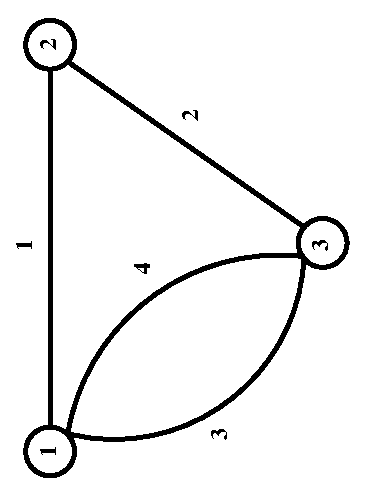
\psfig{file=graph3.ps,angle=-90}}
  \caption{Small undirected graph}
  \label{fig-usmall}
\end{figure}

Next graph shown in figure~\ref{fig-isolated} is directed and has one
isolated node (number 3): 
\begin{verbatim}
g=make_graph('foo',1,4,[1,2,4,1],[2,4,1,4]);
\end{verbatim}

\begin{figure}
  \centerline{\psfig{file=graph4.ps,angle=-90}}
  \caption{Isolated node in directed graph}
  \label{fig-isolated}
\end{figure}

But what about the other elements of the graph-list (see \ref{graph-list})? 
In fact, you do not need to give them if they
are meaningless for your problem or you do not know what to put. Defaults
are given for you. The only needed elements are the arguments of the
\T{make-graph} function:
\begin{description}
  \item[name] the name of the graph
  \item[directed] 0 or 1 according to the fact that the graph is
    respectively undirected or directed
  \item[node\_number] the number of nodes of the graph
  \item[tail] the vector of the  tail node numbers of the graph (its
    size is the number of edges of the graph)
  \item[head] the vector of the head node numbers of the graph (its 
    size is the number of edges of the graph)
\end{description}

and the type \T{'graph'} as the
first element of the list.

All the other elements can be given as the empty vector \T{[]}. Then
defauls are automatically chosen. These defaults are given in the
description of the graph-list (see \ref{graph-list}).

But you can also create your own graph-list by hands, without using the 
\T{make\_graph} function. For that you can use the Scilab function
\T{list}
directly and modify it with the insertion list functions. This way can lead
to errors, because the list is somehow long. You can use the 
\T{check\_graph}
function to check if a Scilab variable can represent a graph-list.

\section{Graph Computations}

\chapter{XMetanet}\label{XMetanet}

\section{Graph Files}

\chapter{Graph List}\label{graph-list}
\index{graph list}
A graph in Scilab is represented by a Scilab typed list with 32 elements. 
We call it a
graph-list.

You will find below the complete description of the list.

Each element is described by two or more lines.
The first line gives the order of the element in the list and its name.
The other lines give the meaning of the element with its Scilab type if
needed.
The last line gives a default for elements that can have one.
Indeed, only the 6 first elements must have a value in the list, all the 
others can be given the empty vector \T{[]} as a value, and then the default 
is used.
For instance, after you have defined a graph-list by
\begin{verbatim}
g=make_graph('min',1,1,1,1);
\end{verbatim}

which is the simplest graph you can create in Metanet (it is directed, has 
one node and one loop arc on this node), the value of \T{g} is:
\begin{verbatim}
list('graph','min',1,1,1,1,[],[],[],[],[],[],[],[],[],[],[],[],[],[],[],
     [],[],[],[],[],[],[],[],[],[],[],[])
\end{verbatim}

The name of the element is very important because it is used to access 
the elements
of the list. For instance, if \T{g} is a graph-list, to get the name
of the graph, you only have to execute:
\begin{verbatim}
g('name')
\end{verbatim}

and if you want to change the name of the graph to \T{'toto'} for
instance, you have to execute: 
\begin{verbatim}
g('name')='toto';
\end{verbatim}

\begin{enumerate}
  \item \T{type}

the type of the list; it must always be \T{'graph'}

  \item \T{name} 

the name of the graph; a string with a maximum of 80 characters

  \item directed 

flag equal to 1 if the graph is directed or equal to 0 is the graph is
undirected 

  \item \T{node\_number}

number of nodes

  \item \T{tail}

vector of the tail node numbers

  \item \T{head}

vector of the head node numbers

  \item \T{node\_name}

vector of node names

default is the node numbers as node names

  \item \T{node\_type}

vector of the node types; the type is an integer from 0 to 2:
\begin{itemize}
  \item[0:] plain node
  \item[1:] sink node
  \item[2:] source node
\end{itemize}


default is 0 (plain node)

  \item \T{node\_x}

vector of the x coordinate of the nodes

default is computed

  \item \T{node\_y}

vector of the y coordinate of the nodes

default is computed

  \item \T{node\_color}

vector of the node colors; 
the color is an integer from 0 to 16:
\begin{itemize}
  \item[0:] black
  \item[1:] navyblue
  \item[2:] blue
  \item[3:] skyblue
  \item[4:] aquamarine
  \item[5:] forestgreen
  \item[6:] green
  \item[7:] lightcyan
  \item[8:] cyan
  \item[9:] orange
  \item[10:] red
  \item[11:] magenta
  \item[12:] violet
  \item[13:] yellow
  \item[14:] gold
  \item[15:] beige
  \item[16:] white
\end{itemize}


default is 0 (black)

  \item \T{node\_diam}

vector of the size of the node diameters in pixels (a node is
drawn as a circle) 

default is the value of element \T{default\_node\_diam}

  \item \T{node\_border}

vector of the size of the node borders in pixels (a node is drawn
as a circle) 

default is the value of element \T{default\_node\_border}

  \item \T{node\_font\_size}

vector of the size of the font used to draw the name of the node; 
you can choose
8, 10, 12, 14, 18 or 24

default is the value of element \T{default\_font\_size}

  \item \T{node\_demand}

vector of the node demands

default is 0

  \item \T{edge\_name}

vector of the edge names

default is the edge numbers as edge names

  \item \T{edge\_color}

vector of the edge colors; 
the color is an integer from 0 to 16 (see \T{node\_color})

default is 0 (black)

  \item \T{edge\_width}

vector of the size of the edge widths in pixels

default is the value of element \T{default\_edge\_width}

  \item \T{edge\_hi\_width}

vector of the size of the highlighted edge widths in pixels

default is the value of element \T{default\_edge\_hi\_width}

  \item \T{edge\_font\_size}

vector of the size of the font used to draw the name of the edge; you
can choose 8, 10, 12, 14, 18 or 24

default is the value of element \T{default\_font\_size}

  \item \T{edge\_length}

vector of the edge lengths

default is 0

  \item \T{edge\_cost}

vector of the edge costs

default is 0

  \item \T{edge\_min\_cap}

vector of the edge minimum capacities

default is 0

  \item \T{edge\_max\_cap}

vector of the edge maximum capacities

default is 0

  \item \T{edge\_q\_weight}

vector of the edge quadratic weights

default is 0

  \item \T{edge\_q\_orig}

vector of the edge quadratic origins

default is 0

  \item \T{edge\_weight}

vector of the edge weights

default is 0

  \item \T{default\_node\_diam}

default size of the node diameters of the graph

default is 20 pixels

  \item \T{default\_node\_border}

default size of the node borders of the graph

default is 2 pixels

  \item \T{default\_edge\_width}

default size of the edge widths of the graph

default is 1 pixel

  \item \T{default\_edge\_hi\_width}

default size of the highlighted edge widths of the graph

default is 3 pixels

  \item \T{default\_font\_size}

default size of the font used to draw the names of nodes and edges

default is 12

\end{enumerate}

\tableofcontents

\listoffigures

\documentclass[11pt]{report}

\textheight=23cm \textwidth=16cm
\topmargin=-1cm
\oddsidemargin=0pt \evensidemargin=0pt \marginparwidth=2cm

\usepackage{psfig}

\newcommand{\T}[1]{{\tt #1}}

\title{Metanet Tutorial}
\author{Claude Gomez \and Maurice Goursat}
\date{14 July 1995}

\makeindex

\begin{document}

\maketitle

Metanet is a toolbox of Scilab. In fact, it is a toolbox of Scilab
with another software linked to Scilab: XMetanet.

The Scilab toolbox consists of fortran and C programs and Scilab
macros.  
They give a set of Scilab functions dealing with graph and
network computations. A new object, a graph-list is defined in Scilab to handle
graph.

XMetanet is a X Window application for creating, modifying and
vizualizing graphs and networks. XMetanet and Scilab can be
used separately. 

 The first chapter is a tutorial which explains
how to use the Metanet toolbox of Scilab.
 The second chapter describes explains how to use the X
Window application XMetanet.
 The third chapter describes the structure of the
graph-list.
 The last chapter describes all the functions
of the toolbox.

\chapter{Using Metanet}

You can use the Metanet toolbox in Scilab without using XMetanet window at
all,
\mbox{i.e.} without seeing the graphs or the networks you are working with,
even if it seems better to use XMetanet to see them. You only need to use 
XMetanet when you want to see graphs, or when you want to load already 
saved graph.
So, a good thing to do before using Metanet
is to open a Metanet window, \mbox{i.e.} to execute the X Window application
XMetanet from Scilab. For that, use the Metanet Menu in
Scilab. It is exactly the same as issuing the command \T{metanet()}.

\section{Creating and Loading Graphs}

A graph in Scilab is defined by a list: we call it a
{\em graph-list}. It  
is described in \ref{graph-list}. This list contains everything needed to
define the graph, from the arcs and nodes to the color and width of the
arcs. We are going to see it is not necessary to fill of the elements of
the list; for most of them defaults are given.

To create a new graph in Scilab, you can make a new graph-list or make the
graph by using XMetanet and load it. We describe her
the first way: make a new graph-list. For the second way, see \ref{XMetanet}.
For making a graph-list, use the
\T{make\_graph} function.

For instance, the directed graph named ``foo'' in figure~\ref{fig-small}
has three nodes and four
arcs. We call \T{g} the corresponding graph-list.

\begin{figure}
  \centerline{\psfig{file=graph1.ps,angle=-90}}
  \caption{Small directed graph}
  \label{fig-small}
\end{figure}

You can easily create it by issuing the command:

\begin{verbatim}
g=make_graph('foo',1,3,[1,2,3,1],[2,3,1,3]);
\end{verbatim}

The first argument is the name of the graph,
the second argument \T{1} says that the graph is directed, the third
and fourth arguments are what we call tail
and head
vectors of 
the graph and the last argument is the number of nodes of the graph.

To understand this, we need to explain how a graph is represented.

The graphs handled by Metanet are directed or undirected multigraphs 
(loops are allowed). 
A {\em graph}\index{graph}
is a set of arcs and nodes. A graph must at least have one arc. 
We call {\em arc}\index{arc} a directed link between two nodes. 
For instance the arc $(i,j)$ goes from the {\em tail}\index{tail}
node $i$ to the {\em head}\index{head}
node $j$. 
We call {\em edge}\index{edge} the 
corresponding undirected link. A minimal way to represent a graph is to
give the number of nodes, the list of the tail nodes and the list of the
head nodes. Each node has a number and each arc has a number. The numbers
of nodes are consecutive and the number of arcs are consecutive. In Scilab,
these lists are represented by vectors. So, if we call \T{tail} and
\T{head} these vectors, the arc number $i$ goes from node
number \T{tail(i)} to node number \T{head(i)}. Moreover, the number of
nodes is necessary, because isolated nodes (without any arc) can exist. The
size of the vectors tail and head is the number of edges of the graph.

The distinction between edges and arcs is meaningful when we deal with
undirected graphs. In computations, an undirected graph is considered as a
directed graph where each edge of the undirected graph is splitted into two
arcs with consecutive numbers: the edge  number $u$ between nodes $i$ and $j$
becomes the arc  number $2i-1$ from node $i$ to node $j$ and the arc 
 number
$2i$ from node $j$ to node $i$. This distinction is not needed when we
only use the standard functions of Metanet.

The simplest graph we can create in Metanet is:
\begin{verbatim}
g=make_graph('min',1,1,1,1);
\end{verbatim}

It is directed, has one node and one loop arc on this node and can be
seen in figure~\ref{fig-smallest}.
\begin{figure}
  \centerline{\psfig{file=graph2.ps,angle=-90}}
  \caption{Smallest directed graph}
  \label{fig-smallest}
\end{figure}

The following graph shown in figure~\ref{fig-usmall} is the same as
the first graph we have created, but it 
is undirected:
\begin{verbatim}
g=make_graph('foo',0,3,[1,2,3,1],[2,3,1,3]);
\end{verbatim}

\begin{figure}
  \centerline{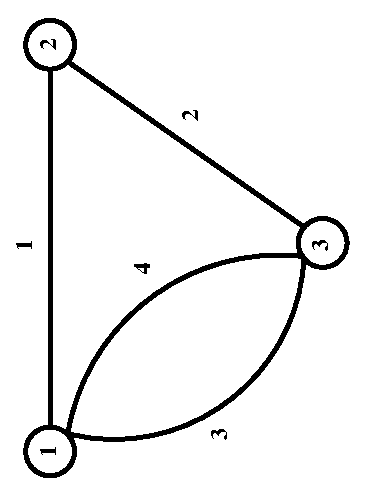
\psfig{file=graph3.ps,angle=-90}}
  \caption{Small undirected graph}
  \label{fig-usmall}
\end{figure}

Next graph shown in figure~\ref{fig-isolated} is directed and has one
isolated node (number 3): 
\begin{verbatim}
g=make_graph('foo',1,4,[1,2,4,1],[2,4,1,4]);
\end{verbatim}

\begin{figure}
  \centerline{\psfig{file=graph4.ps,angle=-90}}
  \caption{Isolated node in directed graph}
  \label{fig-isolated}
\end{figure}

But what about the other elements of the graph-list (see \ref{graph-list})? 
In fact, you do not need to give them if they
are meaningless for your problem or you do not know what to put. Defaults
are given for you. The only needed elements are the arguments of the
\T{make-graph} function:
\begin{description}
  \item[name] the name of the graph
  \item[directed] 0 or 1 according to the fact that the graph is
    respectively undirected or directed
  \item[node\_number] the number of nodes of the graph
  \item[tail] the vector of the  tail node numbers of the graph (its
    size is the number of edges of the graph)
  \item[head] the vector of the head node numbers of the graph (its 
    size is the number of edges of the graph)
\end{description}

and the type \T{'graph'} as the
first element of the list.

All the other elements can be given as the empty vector \T{[]}. Then
defauls are automatically chosen. These defaults are given in the
description of the graph-list (see \ref{graph-list}).

But you can also create your own graph-list by hands, without using the 
\T{make\_graph} function. For that you can use the Scilab function
\T{list}
directly and modify it with the insertion list functions. This way can lead
to errors, because the list is somehow long. You can use the 
\T{check\_graph}
function to check if a Scilab variable can represent a graph-list.

\section{Graph Computations}

\chapter{XMetanet}\label{XMetanet}

\section{Graph Files}

\chapter{Graph List}\label{graph-list}
\index{graph list}
A graph in Scilab is represented by a Scilab typed list with 32 elements. 
We call it a
graph-list.

You will find below the complete description of the list.

Each element is described by two or more lines.
The first line gives the order of the element in the list and its name.
The other lines give the meaning of the element with its Scilab type if
needed.
The last line gives a default for elements that can have one.
Indeed, only the 6 first elements must have a value in the list, all the 
others can be given the empty vector \T{[]} as a value, and then the default 
is used.
For instance, after you have defined a graph-list by
\begin{verbatim}
g=make_graph('min',1,1,1,1);
\end{verbatim}

which is the simplest graph you can create in Metanet (it is directed, has 
one node and one loop arc on this node), the value of \T{g} is:
\begin{verbatim}
list('graph','min',1,1,1,1,[],[],[],[],[],[],[],[],[],[],[],[],[],[],[],
     [],[],[],[],[],[],[],[],[],[],[],[])
\end{verbatim}

The name of the element is very important because it is used to access 
the elements
of the list. For instance, if \T{g} is a graph-list, to get the name
of the graph, you only have to execute:
\begin{verbatim}
g('name')
\end{verbatim}

and if you want to change the name of the graph to \T{'toto'} for
instance, you have to execute: 
\begin{verbatim}
g('name')='toto';
\end{verbatim}

\begin{enumerate}
  \item \T{type}

the type of the list; it must always be \T{'graph'}

  \item \T{name} 

the name of the graph; a string with a maximum of 80 characters

  \item directed 

flag equal to 1 if the graph is directed or equal to 0 is the graph is
undirected 

  \item \T{node\_number}

number of nodes

  \item \T{tail}

vector of the tail node numbers

  \item \T{head}

vector of the head node numbers

  \item \T{node\_name}

vector of node names

default is the node numbers as node names

  \item \T{node\_type}

vector of the node types; the type is an integer from 0 to 2:
\begin{itemize}
  \item[0:] plain node
  \item[1:] sink node
  \item[2:] source node
\end{itemize}


default is 0 (plain node)

  \item \T{node\_x}

vector of the x coordinate of the nodes

default is computed

  \item \T{node\_y}

vector of the y coordinate of the nodes

default is computed

  \item \T{node\_color}

vector of the node colors; 
the color is an integer from 0 to 16:
\begin{itemize}
  \item[0:] black
  \item[1:] navyblue
  \item[2:] blue
  \item[3:] skyblue
  \item[4:] aquamarine
  \item[5:] forestgreen
  \item[6:] green
  \item[7:] lightcyan
  \item[8:] cyan
  \item[9:] orange
  \item[10:] red
  \item[11:] magenta
  \item[12:] violet
  \item[13:] yellow
  \item[14:] gold
  \item[15:] beige
  \item[16:] white
\end{itemize}


default is 0 (black)

  \item \T{node\_diam}

vector of the size of the node diameters in pixels (a node is
drawn as a circle) 

default is the value of element \T{default\_node\_diam}

  \item \T{node\_border}

vector of the size of the node borders in pixels (a node is drawn
as a circle) 

default is the value of element \T{default\_node\_border}

  \item \T{node\_font\_size}

vector of the size of the font used to draw the name of the node; 
you can choose
8, 10, 12, 14, 18 or 24

default is the value of element \T{default\_font\_size}

  \item \T{node\_demand}

vector of the node demands

default is 0

  \item \T{edge\_name}

vector of the edge names

default is the edge numbers as edge names

  \item \T{edge\_color}

vector of the edge colors; 
the color is an integer from 0 to 16 (see \T{node\_color})

default is 0 (black)

  \item \T{edge\_width}

vector of the size of the edge widths in pixels

default is the value of element \T{default\_edge\_width}

  \item \T{edge\_hi\_width}

vector of the size of the highlighted edge widths in pixels

default is the value of element \T{default\_edge\_hi\_width}

  \item \T{edge\_font\_size}

vector of the size of the font used to draw the name of the edge; you
can choose 8, 10, 12, 14, 18 or 24

default is the value of element \T{default\_font\_size}

  \item \T{edge\_length}

vector of the edge lengths

default is 0

  \item \T{edge\_cost}

vector of the edge costs

default is 0

  \item \T{edge\_min\_cap}

vector of the edge minimum capacities

default is 0

  \item \T{edge\_max\_cap}

vector of the edge maximum capacities

default is 0

  \item \T{edge\_q\_weight}

vector of the edge quadratic weights

default is 0

  \item \T{edge\_q\_orig}

vector of the edge quadratic origins

default is 0

  \item \T{edge\_weight}

vector of the edge weights

default is 0

  \item \T{default\_node\_diam}

default size of the node diameters of the graph

default is 20 pixels

  \item \T{default\_node\_border}

default size of the node borders of the graph

default is 2 pixels

  \item \T{default\_edge\_width}

default size of the edge widths of the graph

default is 1 pixel

  \item \T{default\_edge\_hi\_width}

default size of the highlighted edge widths of the graph

default is 3 pixels

  \item \T{default\_font\_size}

default size of the font used to draw the names of nodes and edges

default is 12

\end{enumerate}

\tableofcontents

\listoffigures

\input{metanet.ind}

\end{document}


\end{document}


\end{document}


\end{document}
